\section{Thuật toán Berry-Ravindran}

\subsection{Đặc điểm chính}

Thuật toán Berry-Ravindran là sự kết hợp giữa hai thuật toán Quick Search và Zhu-Takaoka nhằm cải thiện hiệu quả của phép dịch chuyển bad-character. Thuật toán sử dụng đồng thời hai ký tự liên tiếp nằm ngay bên phải cửa sổ hiện tại của văn bản để xác định khoảng dịch chuyển, nhờ đó thường tạo được các bước nhảy lớn hơn trong thực tế.

Berry-Ravindran kế thừa ý tưởng dịch chuyển nhanh của Quick Search và cơ chế xét cặp ký tự của Zhu-Takaoka, từ đó đạt hiệu năng tốt trên nhiều loại dữ liệu văn bản khác nhau.

Thuật toán có các đặc điểm sau:
\begin{itemize}
    \item là sự kết hợp của thuật toán Quick Search và Zhu-Takaoka;
    \item giai đoạn tiền xử lý có độ phức tạp thời gian và không gian $O(m + \sigma ^ 2)$;
    \item giai đoạn tìm kiếm có độ phức tạp thời gian $O(mn)$.
\end{itemize}

\subsection{Mô tả thuật toán}

Berry và Ravindran đã thiết kế một thuật toán thực hiện phép dịch chuyển bằng cách xét phép dịch chuyển bad-character cho hai ký tự liên tiếp của văn bản nằm ngay bên phải cửa sổ hiện tại (xem thuật toán Boyer-Moore).

Giai đoạn tiền xử lý của thuật toán bao gồm việc tính toán, với mỗi cặp ký tự $(a, b)$, trong đó $a,b \in \Sigma$, lần xuất hiện ngoài cùng bên phải của chuỗi $ab$ trong chuỗi $axb$.

Với $a,b \in \Sigma$:

\[
brBc[a,b]
=
\min \left\{
\begin{array}{ll}
1 & \text{nếu } x[m - 1] = a, \\

m - i + 1 & \text{nếu } x[i]x[i+1] = ab, \\

m + 1 & \text{nếu } x[0] = b, \\

m + 2 & \text{trong trường hợp còn lại.}
\end{array}
\right.
\]

Giai đoạn tiền xử lý có độ phức tạp thời gian và không gian $O(m + \sigma ^ 2)$.

Sau mỗi lần thử khi cửa sổ được đặt trên đoạn văn bản $y[j \dots j + m - 1]$, thuật toán thực hiện phép dịch chuyển có độ dài bằng:

\[
brBc[y[j+ m], y[j + m + 1]].
\]

Ký tự $y[n]$ được gán bằng ký tự rỗng (null character), và $y[n+ 1]$ cũng được gán bằng ký tự này để có thể tính toán các phép dịch chuyển cuối cùng  của thuật toán.

Giai đoạn tìm kiếm của thuật toán Berry-Ravindran có độ phức tạp thời gian $O(mn)$.

\subsection{Cài đặt bằng C++}
\begin{verbatim}
#include <iostream>
#include <vector>
#include <string>
#include <cstring>

using namespace std;

const int ASIZE = 256;

/* Preprocessing: Berry-Ravindran Bad Character Table */
void preBrBc(const string &pat,
             vector<vector<int>> &brBc) {
    int m = pat.length();

    brBc.assign(ASIZE, vector<int>(ASIZE, m + 2));

    for (int a = 0; a < ASIZE; ++a) {
        brBc[a][(unsigned char)pat[0]] = m + 1;
    }

    for (int i = 0; i < m - 1; ++i) {
        brBc[(unsigned char)pat[i]]
             [(unsigned char)pat[i + 1]]
            = m - i;
    }

    for (int a = 0; a < ASIZE; ++a) {
        brBc[(unsigned char)pat[m - 1]][a] = 1;
    }
}

/* Berry-Ravindran Algorithm */
void BR(const string &pat, const string &text) {
    int m = pat.length();
    int n = text.length();

    vector<vector<int>> brBc;

    /* Preprocessing */
    preBrBc(pat, brBc);

    /* Add two sentinel characters */
    string txt = text + "\0\0";

    /* Searching */
    int j = 0;

    while (j <= n - m) {

        if (memcmp(pat.c_str(),
                   txt.c_str() + j,
                   m) == 0) {
            cout << "Pattern found at index: "
                 << j << endl;
        }

        j += brBc[
            (unsigned char)txt[j + m]
        ][
            (unsigned char)txt[j + m + 1]
        ];
    }
}

int main() {
    string text = "ABAAABCDABCABC";
    string pattern = "ABC";

    BR(pattern, text);

    return 0;
}
\end{verbatim}

\subsection{Kiểm nghiệm thuật toán}

\textbf{Pha tiền xử lý:}

\begin{center}
    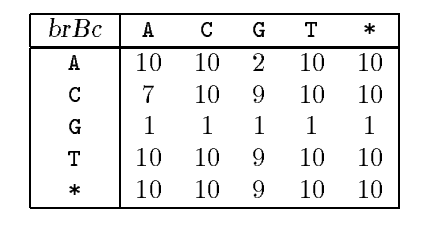
\includegraphics[width=10cm]{Images/2026-05-18-11-07-56.png}
\end{center}

Dấu (*) biểu thị rằng bất kỳ ký tự nào trong $\Sigma \setminus \{A, C, G, T\}$. Bảng $brBc$ được sử dụng bởi thuật toán Berry-Ravindran.

\textbf{Pha tìm kiếm:}

Lần 1:

\begin{center}
    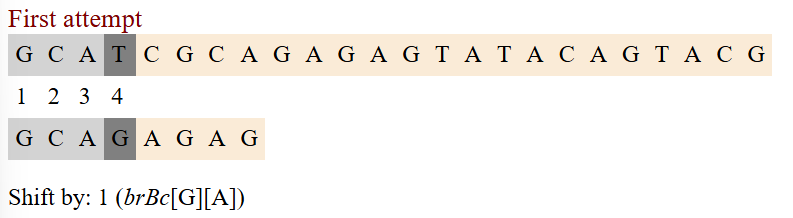
\includegraphics[width=15cm]{Images/2026-05-18-11-10-30.png}
\end{center}

Lần 2:

\begin{center}
    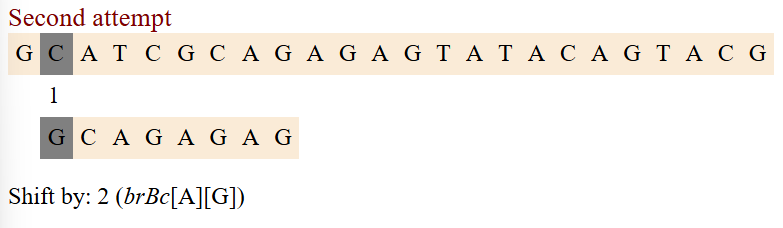
\includegraphics[width=15cm]{Images/2026-05-18-11-10-47.png}
\end{center}

Lần 3:

\begin{center}
    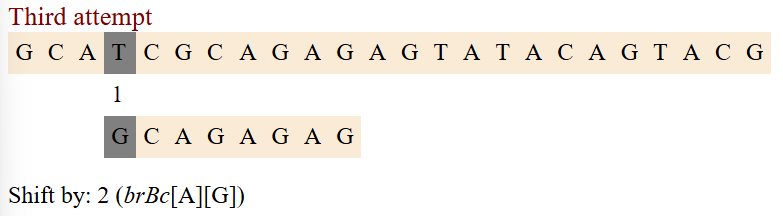
\includegraphics[width=15cm]{Images/2026-05-18-11-11-07.png}
\end{center}

Lần 4:

\begin{center}
    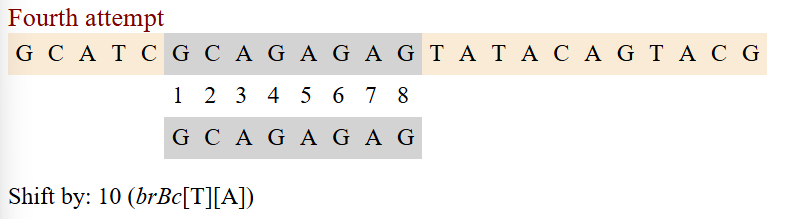
\includegraphics[width=15cm]{Images/2026-05-18-11-11-27.png}
\end{center}

Lần 5:

\begin{center}
    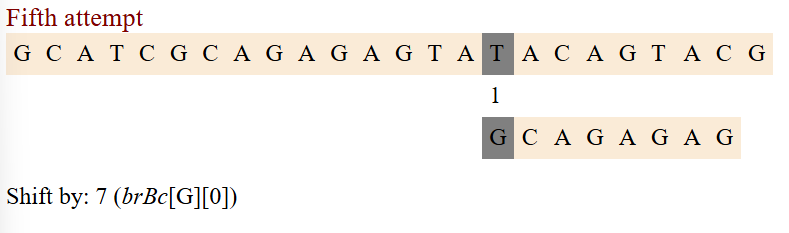
\includegraphics[width=15cm]{Images/2026-05-18-11-11-47.png}
\end{center}

Lần 6:

\begin{center}
    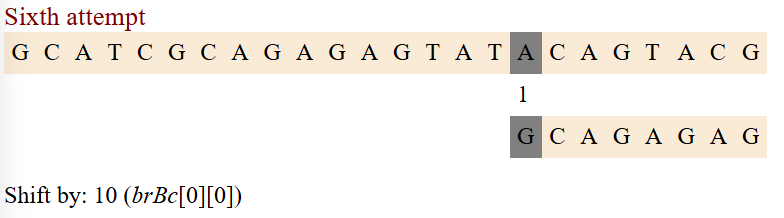
\includegraphics[width=15cm]{Images/2026-05-18-11-12-09.png}
\end{center}

Thuật toán Berry-Ravindran thược hiện 16 phép so sánh ký tự trong ví dụ trên.